\documentclass[letterpaper]{article}

\usepackage{aaai}
\usepackage{prasem}

\begin{document}

\title{Rough Set Semantics for Identity on the Web}
\author{Wouter Beek \and Stefan Schlobach \and Frank van Harmelen\\
Vrije Universiteit Amsterdam\\
De Boelelaan 1081a\\
1081HV Amsterdam\\
The Netherlands}
\maketitle
\begin{abstract}
\begin{quote}
Identity relations are at the foundation of the Linked Open Data initiative
  and on the Semantic Web in general.
They allow the interlinking of alternative descriptions of the same thing.
However, many practical uses of \verb|owl:sameAs| are known to violate its
  formal semantics.
We propose a method that assigns meaning to (the subrelations of)
  an identity relation using the predicates of the dataset schema.
Applications of this approach include automated suggestions for
  asserting/retracting identity pairs and quality assessment.
We also describe an experimental design for this approach.
\end{quote}
\end{abstract}

% Section 1: Introduction
\section{Introduction}
\label{sec:introduction}

Identity relations are at the foundation of the Linked Open Data initiative
  and of the Semantic Web in general \cite{BizerCyganiakHeath2007}.
They allow the interlinking of alternative descriptions of the same thing.
However, the traditional notion of identity
  (expressed by
  {\small \texttt{owl:sameAs}} \cite{MotikPaterschneiderGrau2012})
  is often problematic, e.g. when objects are considered the same in some
  contexts but not in others.
The standing practice in such cases is to use weaker relations of relatedness
  (e.g., {\small \texttt{skos:related}} \cite{MilesBechhofer2009}).
Unfortunately, this limits reasoners in drawing inferences.

According to the traditional semantics of the identity relation,
  identical terms can be replaced for one another in all non-modal contexts
  \emph{salva veritate}.
Practical uses of {\small \texttt{owl:sameAs}} are known to violate this
  strict condition
  \cite{HalpinHayes2010,HalpinHayesMccuskerMcguinnessThompson2010}.

The SW is not only a formal model,
  but is also a social component that evolves over time,
  i.e. it is a social machine \cite{Www2013}.
Being a social and symbolic system at the same time,
  meaning on the SW is denoted by its semantics as well as its pragmatics.

\subsection{Research goals}
\label{sec:research_goals}

In developing our approach we have the following research goals:
\begin{enumerate}
\item In an identity relation the pairs all look the same.
      We want to characterize subrelations of an identity relation in terms
      of the predicates that occur in the schema of the dataset.
\item Based on an existing identity relation we want to give semantically
      motivated suggestions for extending/limiting the identity relation.
\item We want to assess the quality of an identity relation based on
      the consistency with which it is applied to the data.
\end{enumerate}


\subsection{Related work}
\label{sec:related_work}

Existing research proposes six different solutions for
the problem of identity on the Semantic Web.
We now briefly discuss each of these.

Introduce weaker versions of \text{owl:sameAs} and related predicates.
  \cite{halpin_hayes_2010,mccusker_mcguinness_2010}
For example the SKOS concepts \texttt{skos:related}
  which is symmetric but not transitive.
The downside to this approach is that it does not allow transitive inference.

Restrict the applicability of identity relations to specific contexts.
  Identities are expected to hold within a named graph or within a namespace,
  but not necessarily outside of it \cite{halpin_hayes_2010,melo_2013}.
(3) Introduce additional vocabulary that does not weaken but extend
  the existing identity relation \cite{halpin_hayes_2010}.
  For example, allow an explicit distinction to be made between mentioning
  a term and using a term
  (e.g., a car and a Web document describing that car).
(4) Add domain-specific weaker versions of the identity relation
  \cite{mccusker_mcguinness_2010} (e.g., ``have the same medical use''
  is weaker than ``are the same molecule'').
(5) Adapt the modeling practice, possibly in a (semi-)automated way
  by adapting visualization and modeling toolkits to produce notifications
  upon reading SW data, or by posing additional restrictions on the creation
  and alteration of data. For example adding an RDF link could require
  reciprocal confirmation from the maintainers of the respective datasets.
  \cite{halpin_hayes_2010,ding_shinavier_finin_mcguinness_2010}

Other related research focusses on the extraction of network properties of
  \verb|owl:sameAs| datasets \cite{ding_shinavier_shangguan_mcguinness_2010},
  but these endeavors are not yet related to the semantics of the
  identity relation.

What these approaches have is common is that quite some work has to be done
  (adapting or creating standards, instructing modelers, converting existing
  dataset) in order to resolve some of the problems of identity.
Our approach provides a way of dealing with the heterogeneous real-world usage
  of identity in the Semantic Web that is fully automated and that requires
  no changes to standards, modeling practices, or existing datasets.

In modeling the problem arises that identical resources allow reasoning

Since all resources are related

An example from the SW is the property \verb|skos:exactMatch|,
which is used to indicate that two conceptual resources in
different concept schemes are sufficiently similar that
they can be used interchangeably
in an information retrieval application.



% Section 2: Approach
\section{Approach}
\label{sec:approach}

In the following we consider an arbitrary,
  materialized RDF graph $G$ and an identity relation $\sim$ over
  the resources that occur in $G$.
The subject terms of $G$ are denoted by $S_G$, the predicate terms by $P_G$
  and the object terms by $O_G$.

For illustrative purposes we use the IIMB dataset that is used in the
  instance matching track of the 2012 Ontology Alignment Evaluation
  Initiative (OAEI) \cite{oaei_2012}.
This dataset consists of eighty ontologies $G_i$ (for $1 \leq i \leq 80$)
  that are linked to a single base ontology $G_0$.
A graph $G$ is the result of fully materializing the graph merge
  of $G_i$ (for some $1 \leq i \leq 80$) and $G_0$.
For each of these eighty linked ontologies a reference mapping is available.

In RDF a property consists of a single predicate term
  (e.g., the property ``is spoken in'' is denoted by predicate term
   \verb|IIMBTBOX:spoken_in| in the IIMB dataset).
We generalize the notion of a property to consist of
  an arbitrary number of predicate terms.
For this we define a depth-$n$ \emph{predicate path map} (abbr. ppm)
  that is characterized by a sequence of $n$ predicates
  and denotes a (functional) mapping from subject terms
  into sets of object terms
  (def. \ref{def:predicate_path},
   where $p_i \in P_G$ and $[p]_{\sim}$ is the identity set for $p$).
%$f_{\tuple{\range{p_1}{p_n}}}: S_G \rightarrow \mathcal{P}(O_G)$

\small
\begin{definition}[Predicate path map (ppm)]
\begin{align}
\label{def:predicate_path}
  f_{\tuple{\range{p_1}{p_n}}}(s)
\,=\,
  \bigsetdef{o \in O_G}{
    \exists_{\range{x_1}{x_{n-1}}} \quad \quad \quad \quad \quad \quad\\
      \bigwedge_{i=0}^{n-1}\nolimits
          \pair{I(x_i)}{I(x_{i-1})}
        \in
          \bigcup_{p \in [p_{i+1}]_{\sim}}\nolimits \mathit{Ext}(I(p))
  }\nonumber
\end{align}
\end{definition}
\normalsize

\noindent Examples of properties characterized by predicate path maps are
  ``is spoken in'' (depth-$1$) and
  ``is spoken in a country whose form of government is'' (depth-$2$).


% Section 3: Experiments
\section{Experimental design}
\label{sec:experimental_design}

For illustrative purposes we use the IIMB dataset that is used in the
  instance matching track of the 2012 Ontology Alignment Evaluation
  Initiative (OAEI\footnote{\URL{oaei.ontologymatching.org}}).
This dataset consists of eighty ontologies $G_i$ (for $1 \leq i \leq 80$)
  that are linked to a single base ontology $G_0$.
The identity links between $G_0$ and $G_i$ are annotated with a
  confidence measure between $0.0$ and $1.0$.
A graph $G$ is the result of fully materializing the graph merge
  of $G_i$ (for some $1 \leq i \leq 80$) and $G_0$.
For each of these eighty linked ontologies a reference mapping is available.



\subsection{Experimental results}

In this experiment we incrementally remove part of the identity relation.
We then calculate the rough set representation using this altered relation.
We then evaluate how many of the removed identity pairs occur in
  the higher approximation.
Our hypothesis is that the percentage of removed identity pairs
  in the higher approximation is higher than the percentage of pairs
  in the higher approximation.
If the hypothesis is validated, this indicates that
  calculating the rough set representation for a partial identity relation
  would indeed improve suggestions for extending that identity relation.

Since the data may contain noise, using precision degrees $0.0$ and $1.0$
  may be too strict. For this experiment we have set these boundaries
  to $0.05$ and $0.95$ respectively.

\begin{figure}
\label{fig:recall_quality}
\centering
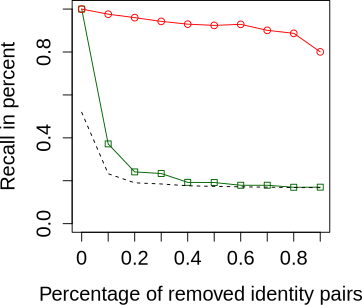
\includegraphics[width=0.8\linewidth]{./img/recall_quality}
\caption{
  The recall of the lower and higher approximation
    are shown by the green and red line respectively.
  The quality metric (definition \ref{def:quality})
    is shown by the dashed line.
}
\end{figure}

\begin{figure}
\label{fig:in_higher}
\centering
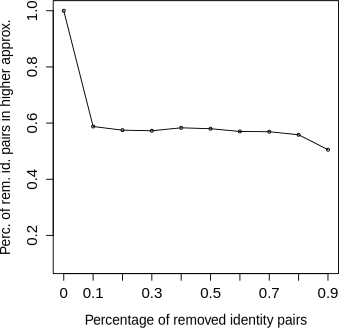
\includegraphics[width=0.8\linewidth]{./img/in_higher}
\caption{
  The percentage of the removed identity pairs that are in the higher approximation
}
\end{figure}

In figure \ref{fig:in_higher}
  we see that the randomly removed identity pairs are often
  in the higher approximation, even when large parts of
  the identity relation are removed.

\begin{comment}
Lower recall
1.0,0.37172100183246687,0.24123550044617229,0.23375413992878838,0.19251810221158194,0.1916729296953922,0.1790536768898471,0.17912482945205316,0.1696252362320524,0.17011849853438268
Higher recall
1.0,0.976185052819561,0.9600384749021372,0.9425765362723856,0.9297564861502547,0.9239282325982691,0.9288077551757412,0.900878631549093,0.886987450993775,0.8005503359226204
Quality
0.5190405227795084,0.23261438049447705,0.1904353344556299,0.18505145463363135,0.17658153004935476,0.17387635867899948,0.17168948193128328,0.17017370794837366,0.16844506704419984,0.1677780567227606
Higher cover
0.0006413304103753317,0.0006098495555258293,0.0005825544051162525,0.0005747252831024628,0.0005640718998200667,0.0005626590987592347,0.0005613753926606205,0.0005464403973849621,0.0005372610299329459,0.00046916805031848495
Removed identity pairs in higher
1.0,0.5877680311890837,0.5747530425162004,0.572660333493667,0.5831761670185315,0.5799385908868745,0.5701984042084377,0.5692284399224807,0.558405393333526,0.5051324217787632
\end{comment}


\subsection{Hypotheses}
\label{sec:hypotheses}

Since this paper focusses on our novel approach and not on evaluation,
  we will enumerate some of the hypotheses which can be evaluated
  using the here described approach:
\begin{enumerate}
\item Take an {\small \texttt{owl:sameAs}} relation and
        a {\small \texttt{skos:related}}
        relation defined over the same domain.
      Merge them into a new binary relation $\sim$.
      Establishing the lower and higher approximation of $\sim$,
        the hypothesis is that pairs from {\small \texttt{owl:sameAs}}
        occur more frequently in the lower boundary than pairs from
        {\small \texttt{skos:related}},
\item Take a set of alignment pairs, each of which is associated with
        a confidence measure between $0.0$ and $1.0$.
      Choose an arbitrary cutoff point $0.0 < c < 1.0$.
      The hypothesis is that alignments with a confidence larger than $c$
        occur more frequently in the lower approximation than alignments
        with a confidence smaller than $c$.
\item Take a set of automatically generated alignment pairs with
        associated confidence measures and take the gold standard or
        reference alignment for the same dataset.
      The hypothesis is that pairs that occur in the lower approximation
        of the alignment appear relatively more often in the gold standard
        than pairs that occur in the higher approximation of the alignment.
\item The quality measure $\alpha$ of a reference alignment is generally
        higher than the accuracy measure of an automatically generated
        alignment for the same dataset.
      Or, the quality measure is generally higher for identity relations
        that domain experts consider to be correct.
\end{enumerate}

Also, the IIMB datasets are quite small (tens of thousands of triples).
We will have the verify whether the current implementation is able to scale
  to bigger datasets.


% Section 4: Conclusion
\section{Conclusion}
\label{sec:conclusion}

In this paper we have given an new approach for characterizing,
  extending/retracting, and assessing identity relations.
Our approach does this in purely qualitative terms, using schema semantics.
In contemporary ontology alignment and data linking activities nonsemantic
  aspects of resources play a role as well.
For instance similarity assessment for natural language labels is often
  used in data linking.

We think that the qualitative means of characterizing an identity relation
  are a useful addition to existing quantitative means.
Also, we think that it is more useful and viable to enrich existing
  identity relations in the LOD based on the semantics of the datasets
  in which they occur, than to introduce new relationships into SW languages.
Apart from the practical difficulties of teaching practitioners
  and transforming/enriching existing datasets, we suggest that the
  meaning of an identity (sub)relation is partially defined in its use,
  i.e., in the indiscernibility criteria it embodies.

For our approach it is not necessary to pose additional restrictions
  on a binary relation $\sim$.
The definitions in this paper apply to \verb|owl:sameAs| relations
  in the same way in which they apply to any other binary relation
  (e.g., \verb|skos:related|).

We are currently in the process of validating the above enumerated hypotheses.
The results of these evaluations are continuously being published on
  \verb|wouterbeek.com/identity-on-the-web|.
The website currently contains the automated results of all eighty IIMB
  alignments, drawn from the instance matching track of the
  OAEI 2012.
The website also refers to the publicly available Git repository
  \verb|github.com/wouterbeek/IOTW| where the implementation
  discussed in section \ref{sec:implementation} can be found.

%\input{./tex/futurework.tex}

% Bibliography
\bibliographystyle{aaai}
\bibliography{kr2014_iotw}

\end{document}
